\documentclass{llncs}
\usepackage[utf8]{inputenc}
\usepackage{todonotes}
\usepackage{amsmath}
\usepackage{textcomp} % for \textdegree
\usepackage[hidelinks]{hyperref}
\usepackage{cleveref}
\crefname{figure}{Fig.}{Fig.}
\usepackage{xstring}
\usepackage{booktabs}
\usepackage{tikz}
\usetikzlibrary{arrows,snakes,patterns,matrix,shapes,fit,calc,shadows,plotmarks,decorations.pathmorphing,decorations.markings,backgrounds}
\usetikzlibrary{external}
\tikzexternalize
\tikzsetexternalprefix{fig/}

\usepackage{pgfplots}
\pgfplotsset{compat=1.4, width=0.9\columnwidth, height=0.6\columnwidth}

\newcommand{\inputtikz}[1]
{
  \StrSubstitute{#1}{/}{.}[\fn]
  \scancs{\filename}{\fn}
  \tikzsetfigurename{\filename}
  \input{#1.tikz}
}

\graphicspath{{fig/}}
%%%%%%%%%%%%%%%%%%%%%%%%%%%%%%%%%%%%%%%%%%%%%%%%%%%%%%%%%%%%%%%%%%%%%%%%%%%%%%%%
\begin{document}

\title{SimSpark: An Open Source Robot Simulator Developed by RoboCup Community}

\author{Yuan Xu\inst{1} \and Hedayat Vatankhah\inst{2}}

\institute{
\begin{minipage}[t]{0.4\textwidth}
\centering
DAI-Labor \\
Technische Universität Berlin \\
Ernst-Reuter-Platz 7, Berlin \\
D-10587 Germany\\
\email{yuan.xu@dai-labor.de}
\end{minipage}
\begin{minipage}[t]{0.4\textwidth}
\and
\centering
Amirkabir University of Technology, Iran\\
\email{hedayatv@gmail.com}
\end{minipage}
}

\maketitle

\begin{abstract}
  - current state of simspark
  - changes 2013
  - evidence of impact of the released component to the RoboCup community.
  - technical contribution
  - benefit for the RoboCup community.
\end{abstract}

\section{Introduction}
The development on robots may be severely limited by the constrained resources.
This is especially true in the research of multi-robots systems in areas such as RoboCup.
Using simulation for algorithm development and testing makes thing easier.

% \paragraph{History}
\textit{SimSpark}, a multi-robot simulator based on the generic components of the Spark\cite{OR05} physical multi-agent simulation system, has been used in the RoboCup Soccer Simulation League since 2004.
The project was registered as open source project in SourceForge\footnote{\url{http://simspark.sourceforge.net}} in 2004, it has an established code base with development increasing year-over-year.
As the result, RoboCup soccer simulations have changed significantly over the years, going from rather abstract agent representations to more and more realistic humanoid robot games\cite{Boedecker2008,usermanual}.
Thanks to the flexibility of the Spark system, these transitions were achieved with little changes to the simulator’s core architecture.

In this paper we describe the recent development of \textit{SimSpark} project, which make the \textit{SimSpark} possible to simulate 11 vs. 11 humanoid robot soccer games in real time\todo{is it real time in RoboCup?}.
In section \ref{s:overview}, we will give an overview of \textit{SimSpark} project since 2008. After that, we will describe the development in core module -- names \textit{Spark} in section \ref{s:spark}. In section \ref{s:rcssserver3d}, we will give the implementation of RoboCup 3D Soccer Simulator -- \textit{RCSSServer3D}. We will introduce some ongoing work for RoboCup 2013 in 
section \ref{s:ongoing}. Furthermore, we will discuss the application of \textit{SimSpark} not only in simulation league but also other leagues with real robots in section \ref{s:application}. Finally, we will outline future development plans in section \ref{s:conclusion} .

\todo[inline,color=gray]{Releated work: SimRobot, Webots, V-REP, Gazebo...}


\section{Project Overview}
\label{s:overview}
Because last paper about simspark was in 2008

In comparison to specialized simulators, users can create new simulations by using a scene description language.

Agents communicate with the simulation server via UDP or TCP, and therefore can be implemented in any language that supports such sockets.\todo{integrated agent as well}
Multiple software agents can participate in one simulation.

Simulations are created within the server using the Ruby language and text-based RSG files.
SimSpark uses the Open Dynamics Engine (ODE) for detecting collisions and for simulating rigid body dynamics. ODE allows accurate simulation of the physical properties of objects such as velocity, inertia and friction.

The soccer simulation for this tournament was developed in parallel with the SimSpark simulator. In its initial version players were modeled as spheres in a physical three dimensional world. Since then SimSpark grew considerably and now supports humanoid players with articulated bodies.

% \subsection{Architectural Changes (?)}
\todo[inline]{separation of simspark and rcssserver3d}\todo{Hedayat Vatankhah:
Architecture Enhancements Proposal for Soccer Simulation Server 3D}
It served from the beginning as a test bed and a guide for essential new features that were added to the simulator during development. However changes to the simulator core were never customized for the soccer simulation. Instead generic simulator services were implemented with all soccer specific details contained in a set of plugins.

\todo[inline]{Cmake migration?}
\todo[inline]{windows support (mingw32,VC)}

\section{Spark}
\label{s:spark}
\subsection{New Sensors}
 - ACC
 - FSR
 - Gyro
 - Restrict Vision
 -- Line perceptions
 -- camera (image)

\todo[inline]{sync mode (simspark)}
\todo[inline]{integrated agents (simspark)}
\todo[inline]{physics simulation engine abstraction (simspark)}

\paragraph{Multi-threads Supporting\todo{agent controls}}
In modern time, computers have a CUP with multi-cores or even multi-CPUs.
This improves the performance greatly, but only the multi-threaded program can benefit.
One great feature of SimSpark is switching between single thread mode and multi-threads
mode. The multi-threads mode can improve the performance in computer with multi-cores CPU, but the single thread mode is also useful for developing the simulator. 

The implementation of multi-threads loop is based on two conditions.
First, different tasks are assigned to different \textit{SimControlNode}s in SimSpark.
For example, \textit{AgentControl} is a node that manages the communication with agents.
For each simulation cycle, \textit{SimControlNode}s are executed one by one in the single thread mode, but they can run in parallel.
Second, all data of simulation state is stored in a tree called \textit{active scene},
the physics engine and \textit{SimControlNode}s interact through the \textit{active scene}.
As we know, the physics computation is the most time-consuming, and the physics engine does not need to access the active scene during physics computation.
So the physics computation and \textit{SimControlNode}s can run in parallel.\todo[color=green]{UML?}\todo[color=yellow]{results of performance improvement, any benchmark?}

\todo[inline]{
Sander van Dijk and Ubbo Visser
Proposal: Boosting the 3D SSL Simulator
Increase Research Possibilities in the RC SSL Community

ODE TBB, ??sander's paper -- where??}\footnote{\url{http://www.robocup.org/2011/03/robocup-federation-call-for-project-proposals-2/}}

\todo[inline]{Internal/External Monitor}

\todo[inline]{logfiles}

\section{RCSSServer3D}
\label{s:rcssserver3d}
\todo[inline]{robot model: NAO (rcssserver3d)}
\todo[inline]{soccer rules (referee) (rcssserver3d)}
\todo[inline]{bigger fields and more robots (rcssserver3d)}

\section{Experimental Features}
\label{s:ongoing}
These features are experimental, they (probably) will be used in RoboCup 2013 for the first time. (Some of them are still under the development)

\subsection{Realistic Motor}
\todo{motivation: my email...}
\todo{shorter}
NAO robot has twenty-one motor joints as its actuators.
The simple motor model is one reason for the unrealistic simulation results.
The ODE provides a simple model of real life servos.
It has two parameters: a desired speed and the maximum force that is available to reach that speed. The motor brings the body up to speed in one step; and provides force that is not more than is allowed.
There is no motor that works like this in reality.
Furthermore, some aspects like stiffness control, power consumption and temperature regulation, are missing but are also important for robotics.

\paragraph{Stiffness}
The stiffness determines how strong the motor is. The value is from 0.0
to 1.0, 0 means the motor is off and 1 means the motor is running at
full power. In the real robot,
this percentage is the maximum electric current applied to the motor. Setting the
stiffness to 0.5 means that the electric current limitation is reduced
to 50\%.

For a DC motor, the electric current, $I$, determines the output torque,
$\tau$:
\begin{align}
  \tau &= K_\tau I \label{eq:tau-i}
\end{align}
where $K_\tau$ is the torque constant of the motor. It can be found in the
specifications from \cite{naoqi}. In
the simulation, the maximum torque of the servo can be specified, therefore the
stiffness control can be easily implemented by setting the maximum torque
of the simulated servo:
\begin{align}
  \tau_{max}(t) &= k_{s}(t) T_{max}
\end{align}
where $\tau_{max}(t)$ is the maximum torque set in the simulated servo at
time $t$; $k_{s}(t)$ is the stiffness at time $t$; and $T_{max}$
denotes the maximum torque of the servo when stiffness is 1.

\paragraph{Power Consumption}
Another important aspect besides the motor's performance is its
power consumption: how much energy does it cost to run.
The robot is powered by a battery with limited energy, and has to walk during the
game: half a game is 10 minutes.
An even more important factor in energy consumption is
that the motor can overheat if it consumes too much energy and
becomes too hot. In the real NAO, Aldebaran Robotics estimates the temperature
of each motor by integrating electric current, and shuts down the motor
when the temperature is too high. Therefore modeling power consuming
is important for implementing energy effective motions.

DC motors are based on the following equations:
\begin{align}
  U &= U_e + IR \label{eq:u-ir}\\
  U_e &= K_e \dot{\theta} \label{eq:u-ke}
\end{align}
where $U$ is the voltage of input, $U_e$ is the back electromotive
force (EMF), $I$ is the electric current, $R$ is resistance,
$\dot{\theta}$ is the speed, and $K_e$ is the speed constant of the motor.

The value of $R$ and $K_e$ can be found in the specifications from \cite{naoqi};
and the simulation engine provides
the value of $\tau$ and $\dot{\theta}$; therefore we can calculate the
power consumption by putting \cref{eq:tau-i,eq:u-ir,eq:u-ke} together:
\begin{align}
  P &= UI \\
  &= U_eI + I^2R \\
  &= \frac{K_e}{K_\tau}\dot{\theta}\tau + \frac{R}{K_\tau^2}\tau^2
\end{align}

And the total energy used by the motor is:
\begin{equation}
  \label{eq:motor-power}
  E = \sum_t{P_t\Delta{}t}
\end{equation}
where $\Delta{}t$ is the time step of the simulation, and $P_t$ is the power consumed at time $t$. 

\Cref{fig:battery} compares the simulation result of this model to
reality. In this example, the robot turns left for 5 minutes, then
stands for 1 minutes and then turns right for 5 minutes. This is shown by the change of electric current in the figure. For the overall
power consumption, the energy consumed by devices other than motors,
e.g. mainboard, CPU, camera, etc. has to be added. It is the power
consumption of the robot in an idle state (all motors are off), and measured to be 33 W.

\begin{figure}
  \centering
  \begin{minipage}{0.49\columnwidth}
    \centering
    \pgfplotsset{width=0.9\columnwidth,height=7cm}
    \inputtikz{battery}
    \caption{Power consumption of the real and the simulated robot in action.
      The electric current is the summary of all motors.}
    \label{fig:battery}
  \end{minipage}\hfill{}
  \begin{minipage}{0.49\columnwidth}
    \centering
    \pgfplotsset{width=0.9\columnwidth,height=7cm}
    \inputtikz{joint-temp-LKneePitch}
    \caption{The temperature of the (knee pitch) motor in the simulation and the real robot. The green background is the electric current in the real robot.}
    \label{fig:joint-temperature}
  \end{minipage}
\end{figure}

\paragraph{Temperature Regulation}
We model the temperature and heat of the motor with the following equations:
\begin{align}
  \Delta{}Q^+ &= I^2R\Delta{}t \\
  \Delta{}Q^- &= -\lambda(T-T_e)\Delta{}t \\
  \Delta{}Q &= \Delta{}Q^+ + \Delta{}Q^-\\
  C &= \frac{\Delta{}Q}{\Delta{}T}
\end{align}
where $T$ is the temperature of the motor, $T_e$
is the temperature of the environment, but it is the internal temperature
of motor, so it is higher than outside and differs from motor to
motor, $\Delta{}Q^+$ is the heat produced by the motor, $\Delta{}Q^-$ is
the heat transferred from the motor to the environment, $\Delta{}Q$ is the
heat changing, $\lambda$ is thermal conductivity which indicates the
ability of a motor to conduct heat, and $C$ is the heat capacity of
the motor, which can be seen as constant. Finally, the temperature of
the motor at time $t+\Delta{}t$ can be solved as:
\begin{equation}
  \label{eq:motor-temp}
  T_{t+\Delta{}t} = T_t + \Delta{}T = T_t + \frac{[I^2R-\lambda(T_t-T_e)]\Delta{}t}{C}
\end{equation}

In this model, we determined $T_e$, $\lambda$, and $C$ by experiments. It can be formulate as a classic linear regression problem. We rewrite \cref{eq:motor-temp} to:
\begin{align}
  \label{eq:motor-temp-ols}
  \Delta{}tx_0 + T_t\Delta{}tx_1 - \Delta{}t x_2 &= I^2R \\
  x_0 &= C \\
  x_1 &= \lambda \\
  x_2 &= \lambda Te
\end{align}
A sequence values of $\Delta{}t$, $T_t$, and $I^2R$ can be measured by experiment, therefore the optimum values for $x_0$, $x_1$, and $x_2$ can be obtained by linear least squares method, so the parameters of \cref{eq:motor-temp} is determined. \Cref{tab:motor-parameter} gives the results of the experiment.
\begin{table}[h]
  \centering
  \caption{Parameters $T_e$, $\lambda$ and $C$ in the \cref{eq:motor-temp} for different joints of the NAO V3.}
  \label{tab:motor-parameter}
  \begin{tabular}{lccc}
    \toprule
    Joints      & $T_e$ (\textdegree{}C) & $\lambda$ (W/\textdegree{}C) & $C$ (J/\textdegree{}C)\\
    \midrule
    HipYawPitch & 33 & 0.0158 & 27.2 \\
    \midrule
    HipRoll     & & & \\
    AnkleRoll   & 27 & 0.0158 & 27.2 \\
    \midrule
    HipPitch    & & & \\
    KneePitch   & 27 & 0.0198 & 43.6 \\
    AnklePitch  & & & \\
    \bottomrule
  \end{tabular}
\end{table}

After determining the parameters in the \cref{eq:motor-temp}, we can use this model to simulate motor temperature. In \Cref{fig:joint-temperature}, the simulated temperature is compared with data from the real robot.

The whole process of joint simulation is summarized in
\Cref{fig:joint}: stiffness $k_s$ is simulated by setting the maximum torque
of the motor $\tau_{max}$; the final maximum torque $\tau_m$ used by simulation engine is calculated by temperature regulation; and the simulation engine computes the resulted angle
and torque applied; in the end, the consumed power and temperature are
computed by \cref{eq:motor-power,eq:motor-temp} respectively. When the battery is empty, the maximum torque $\tau_{max}$ is set 0 to turn off the motor.
\begin{figure}
  \centering
  \inputtikz{joint}
  \caption{Pipeline of the servo motor simulation}
  \label{fig:joint}
\end{figure}

\subsection{Heterogeneous Robots}
\todo[inline]{Draft, needs better English}
Simulation is great for experimenting with robots without need to buy expensive 
real robots. Also, the robots are never damaged and they can be used for long 
running experiences without human intervention. 

However, the possibilities which are provided by a simulation environment is 
not limited to these. Not only you can experiment with different behaviors, but
also you can modify the mechanical properties of the robot as you wish. Additionally,
it is possible to create new challenges for robot AI developers since you can
generate robots with different mechanical properties very easily at run time, 
you can provide variations of a robot to teams and they can use them if they can
adopt their developed behaviors to unseen robots; which is in contrast with 
real robots because teams know the exact specification of the robots and
can develop behaviors specifically tuned for a single robot. If heterogeneous 
robots are available in a game, teams can use them only if they can adopt
their behaviors to the robots they didn't know about.

Simspark already provided the ability to define different robot models and 
use them in its simulation environment. However, each model was fixed and if you
wanted to have several variations of a robot, you should have defined several 
separate robot models. To better support games with heterogeneous robots, we have
added the support for parametric models to simspark. Therefore, it is possible to
define models in which a number of parameters are variables and can have different
values for different robot variations.\todo[color=green]{which parameters? for example} When you want to load such a model, you shold 
specify which type of that robot is needed and its parameters are replaced in the
parametric model and the model is created. 

\subsection{Agent Proxies}

\subsection{Player Integration??}

\section{Applications}
\label{s:application}
\paragraph{RoboCup Soccer Simulation League}
In RoboCup 2004, SimSpark was successfully used for the first official competition in RoboCup Simulation 3D League. Since then, it is used as a standard research platform and test bed\todo{How many teams in last RoboCup?}. By using it, simulation teams not only have designed and tested new algorithms, but also developed useful research tools based on SimSpark. Some of these tools are also released as open source.
For example, RoboViz\cite{Stoecker2012} is designed to assess and develop agent behaviors in SimSpark,
it facilitates the real-time visualization of agents running concurrently on the SimSpark simulator,
and provides higher-level analysis and visualization of agent behaviors.

\paragraph{Usage for Real Robot}
As one of the long term goals of the soccer simulation is to aim for realism the long term objective are realistic humanoid players in a physical environment.
These players should one day challenge the champion of the most recent World Cup.
The SimSpark is also used by teams in RoboCup Standard Platform League and Humanoid League.

The special situation between Standard Platform League and 3D Simulation League is that both leagues use the same robot model — NAO from Aldebaran.
So it appears to be natural to reuse the work which has already been done in Simulation League and make SimSpark usable in Standard Platform League.
Nao Team Humboldt developed their software architecture\cite{SCPR2010} which enables their control software can run both in real NAO and simulated NAO with SimSpark. This helps them to achieve some good results in both Simulation League and Standard Platform League.
Furthermore, Nao Team Humboldt also promotes the usage of SimSpark in the Standard Platform League by implementing its rules. \Cref{f:simspark-spl} is the snapshot of the extended SimSpark for Standard Platform League.

\begin{figure}
  \centering
  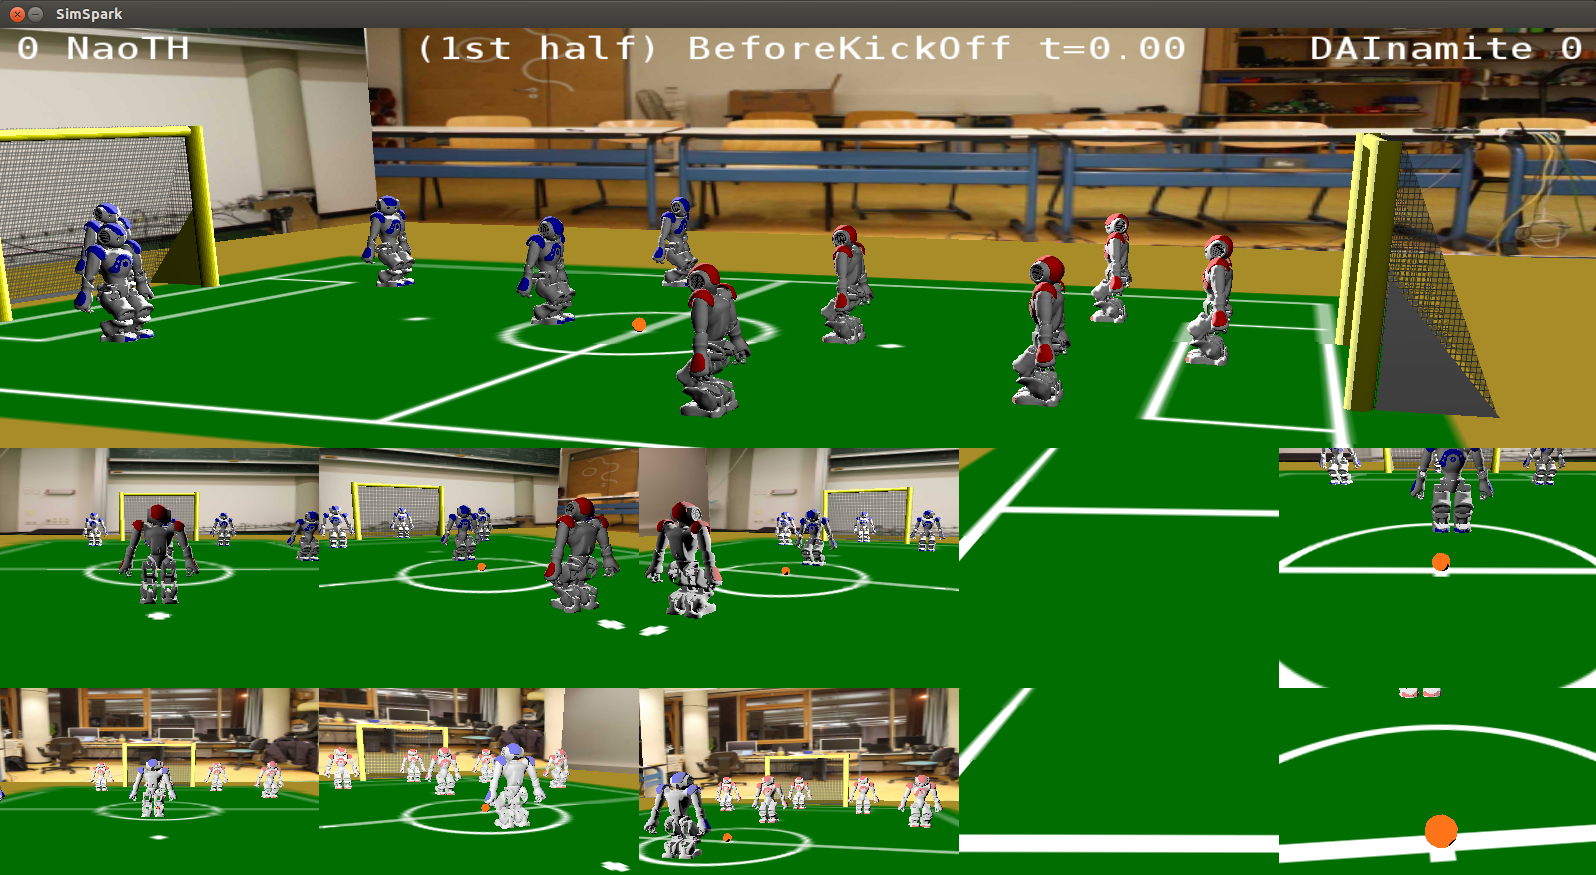
\includegraphics[width = 0.75\columnwidth]{simspark-spl}
  \caption{Prototype of the extended SimSpark for Standard Platform League.
    The bottom of screen are images of robot cameras.}
  \label{f:simspark-spl}
\end{figure}

Of course the simulator can also be extended for other leagues by adding new robot models.
For example, in RoboCup Humanoid Kid Size League, FUmanoid\cite{Donat2012} uses
SimSpark to perform multi-level testing methods for archiving higher
quality in each module of their robot control software and unlink the
module test from the robotic hardware.


\section{Conclusion and Future Work}
\label{s:conclusion}
SimSpark is a powerful tool to state different multi-agent research questions.

\todo[inline]{Other physic engine, Bullet}
\todo[inline]{better GUI}

\section*{Acknowledgments}

\bibliographystyle{splncs03}
\bibliography{reference}
\end{document}
